\section{Declarative goals and domain properties\label{section:background-goals}}

A \emph{goal} is a prescriptive statement of intent, whose satisfaction requires the collaboration of agents forming the system. Unlike goals, \emph{domain properties} are descriptive statement about the environment -- such as physical laws, organizational rules, etc. Goals are structured in AND/OR refinement graphs showing how they contribute to each other~\cite{VanLamsweerde:2000}.

Goals and domain properties can be formalized in Linear Temporal Logic (LTL), that allows specifying admissible and/or proscribed system histories in a declarative and implicit way (that is, without requiring an explicit time parameter)~\cite{VanLamsweerde:2009}. In addition to the usual propositional constructs (we ignore first-order constructs here), LTL provides operators for temporal referencing: $\circ$ (at the next smallest time unit), $\diamond$ (some time in the future), $\square$ (always in the future), $\rightarrow$ (implies in the current state), $\Rightarrow$ (always implies), $\mathcal{U}$ (always in the future until), $\mathcal{W}$ (always in the future unless), see~\cite{Manna:1992}.

However, a system history is commonly viewed in LTL as a temporal sequence of system states. Also, atomic propositions of LTL formula often refer to state variables (e.g. in the SPIN model-checker~\cite{Holzmann:1997}). In contrast, a system history is seen as a trace here, that is, a temporal sequence of events. Capitalizing on fluents for reconciling state-based and event-based paradigms (see previous section), we use a flavor of LTL known as Fluent Linear Temporal Logic (FLTL), a linear temporal logic in which atomic propositions are fluents~\cite{Giannakopoulou:2003}. FLTL proves a convenient way for specifying state-based temporal logic properties over the event-based operational model given by our scenarios and state machines. For example, the safety goal ``\emph{Doors shall remain closed while the train is moving}'' of our running example can be formalized in terms of the $Moving$ and $DoorsClosed$ fluents defined in the previous section, as follows:

\begin{center}
\artifact{Maintain[DoorsClosed While Moving]} = $\square(Moving \rightarrow DoorsClosed)$
\end{center}

Properties formalized in temporal logic are often classified as \emph{liveness} or \emph{safety} properties~\cite{Alpern:1986}. The difference between both is generally illustrated with the distinction between ``\emph{something good will eventually happen}'' (liveness) and  ``\emph{something bad never happens}'' (safety). We restrict our attention to safety properties in this thesis. Indeed, reasoning about liveness properties requires considering the acceptance of infinite execution traces, which it ouside the expressiveness of LTSs and regular languages. In contrast, if ``something bad'' happens it must do so after a finite sequence of events, and is irremediable~\cite{Alpern:1986, Giannakopoulou:1999}. Strictly speaking, as with negative scenarios, this is just outside the expressiveness of LTSs, but not of regular languages. Let us explain this by stating the consistency rules first.

\subsubsection*{Multi-view model consistency}

Consider a safety property $G$ and a system $\system$. Let denote by $\mathcal{L}^{-}(G)$ the set of system traces that violates the property. We say that the system respects the property, that is that they are consistent if and only if the following condition holds:

\begin{center}
$\mathcal{L}(Ag_1 \parallel \ldots \parallel Ag_n) \cap \mathcal{L}^{-}(G) = \emptyset$
\end{center}

The equation above simply requires the system not to exhibit traces that violate the safety property. In fact, it is the well known one from model checking~\cite{Clarke:1989}, provided that $\mathcal{L}^{-}(G)$ actually is $\mathcal{L}(\neg G)$, that is the set of traces that satisfy the negation of the safety property. We prefer the former notation here because it is closer to the one used for scenarios, with which goals also have synergetic links. On one side, consistency rules similar to the ones given above exist between safety goals and positive scenarios (given as a collection or a hMSC). They simply express that behaviors illustrated in positive scenarios may not violate safety goals. On the other side, a negative scenario, say $N$, is commonly seen as illustrating the violation of a safety goal, say $G$, if the following condition holds:

\begin{center}
$\mathcal{L}^{-}(N) \subset \mathcal{L}^{-}(G)$
\end{center}

\noindent that is, if the negative traces that it defines are precisely among those prescrived by the safety goal. We know turn to the question of capturing $\mathcal{L}^{-}(G)$ with an automaton.

\subsection{Tester and property automata}

It it straightforward to check that $\mathcal{L}^{-}(G)$ cannot be represented with a pure LTS, because it is not prefix-closed. For example, the trace \artifact{<start open>} certainly violates the safety goal for the train and so, belongs to $\mathcal{L}^{-}(Maintain[DoorsClosed While Moving])$, but \artifact{<start>} does not violate it (yet). However, as a safety property can only be violated after a finite trace and remains violated after that, $\mathcal{L}^{-}(G)$ is suffix-closed. Let contrast this with $\mathcal{L}^{+}(G)$ that denotes the set of all possible system traces that do \emph{not} violate the property. This language certainly includes all traces that, at one event near, do not violate the property; it also includes all their prefixes, but not all their suffixes. That is, $\mathcal{L}^{+}(G)$ is prefix-closed, and can be represented by a LTS. 

In fact, $\mathcal{L}^{-}(G)$ and $\mathcal{L}^{+}(G)$ are \emph{complement} of each other. That is, $\mathcal{L}^{+}(G) = \Sigma^{*} \setminus \mathcal{L}^{-}(G)$. Interestingly, the complement of a regular language is also a regular language~\cite{Hopcroft:1979}, which implies that both can be modeled with standard automata. In contrast, the complement of a prefix-closed language is not prefix-closed, as we have illustrated on the example. Moreover, taking the complement of a language is straightforward as it suffices to flip accepting and non-accepting states of its automaton, provided that the latter has a complete transition function (see Fig.~\ref{image:tester-and-property-automata}). 

\begin{figure}[H]\centering
\scalebox{0.40}{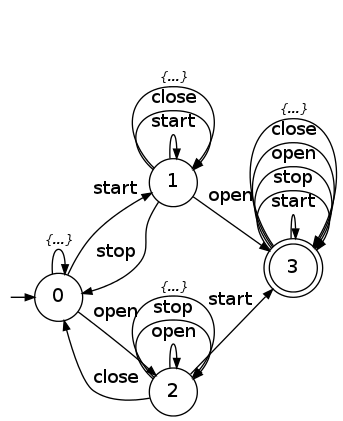
\includegraphics{src/2-framework/images/tester-automaton}}
\scalebox{0.40}{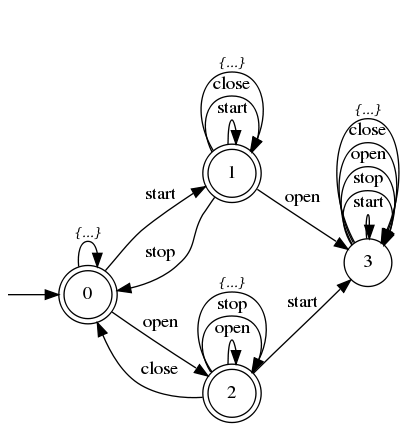
\includegraphics{src/2-framework/images/property-automaton}}
\caption{Tester ($\mathcal{L}^{-}$ at left) and property ($\mathcal{L}^{+}$ at right) automata for \artifact{Maintain[DoorsClosed While Moving]}, as complement of each other.\label{image:tester-and-property-automata}}
\end{figure}

A procedure for computing an automaton capturing $\mathcal{L}^{-}(G)$, called a \emph{tester} automaton for the safety property $G$, is given in \cite{Giannakopoulou:2003}. In short, it consists in composing a b\"uchi automaton that captures the negation of the state-based FLTL property with fluent automata capturing the event-based semantics of fluents, plus a synchronizer between both. Given a pure safety property, a canonical form for this automaton can even been found; the latter is deterministic, has a complete transition function, and a unique sink accepting state capturing all traces (i.e. including all suffixes) violating the property~\cite{Giannakopoulou:2003}. An example of such a tester automaton for the safety goal of the train system is given on the left of~\ref{image:tester-and-property-automata}. One can check that all traces leading to the accepting state model situations where the train is moving with the doors open. The complement of this tester, called here \emph{property} automaton following~\cite{Letier:2005, Letier:2008}, captures $\mathcal{L}^{+}(G)$ and can be obtained by flipping accepting and non-accepting states of the previous one (as shown on the right of the same figure). A few comments are necessary here, though:

\begin{itemize}

\item First, in the LTSA tool \cite{Magee:1999} and related literature, a tester LTS with an error state is used instead of the tester automaton presented here. Similarly, \cite{Letier:2005, Letier:2008} actually uses a property LTS that corresponds to the tester LTS from which the error state has been removed, instead of the property automaton shown here. However, our automata variants are better suited here because of the formalization of inter-model consistency rules, in terms of set-based operators on languages. 

\item More important, the tester and property automata -- and the procedure for computing them in particular -- are always defined ``up to a given alphabet'' or ``under the assumption of a given agent or system''. This is the intended meaning of the transitions labeled ``\emph{\{...\}}" in Fig.~\ref{image:tester-and-property-automata}. The reason is that certain temporal properties, those referring to the \emph{next} operator in particular, are not closed under stuttering~\cite{Lamport:1994}, which means that their satisfaction may be affected by insertion or removal of unobservable events. Which events are relevant depend on additional hypotheses about how goals relate to agent behaviors (e.g. are they under the responsibility of a single agent or are they properties to be respected by the global system). Fixing those ``relevant events'' -- by filling the ``\emph{\{...\}}" placeholders -- is required for respecting the semantics of temporal logic when composing tester and property automata. 

For simplicity in this thesis, we consider that safety properties are to be respected by the global system. Therefore, relevant events are the alphabet of the whole system, say $\Sigma$. Then, a placeholder must be replaced by a transition for each event in $\Sigma$, expect those already labeling an outgoing transition on the same state.

\end{itemize}
